%2multibyte Version: 5.50.0.2960 CodePage: 65001

\documentclass[11pt,letter]{amsart}
%%%%%%%%%%%%%%%%%%%%%%%%%%%%%%%%%%%%%%%%%%%%%%%%%%%%%%%%%%%%%%%%%%%%%%%%%%%%%%%%%%%%%%%%%%%%%%%%%%%%%%%%%%%%%%%%%%%%%%%%%%%%%%%%%%%%%%%%%%%%%%%%%%%%%%%%%%%%%%%%%%%%%%%%%%%%%%%%%%%%%%%%%%%%%%%%%%%%%%%%%%%%%%%%%%%%%%%%%%%%%%%%%%%%%%%%%%%%%%%%%%%%%%%%%%%%
\usepackage{geometry}
\usepackage{graphicx}
\usepackage{amssymb}
\usepackage{epstopdf}
\usepackage{setspace}

\setcounter{MaxMatrixCols}{10}
%TCIDATA{OutputFilter=LATEX.DLL}
%TCIDATA{Version=5.50.0.2960}
%TCIDATA{Codepage=65001}
%TCIDATA{<META NAME="SaveForMode" CONTENT="1">}
%TCIDATA{BibliographyScheme=Manual}
%TCIDATA{LastRevised=Tuesday, February 14, 2017 11:40:11}
%TCIDATA{<META NAME="GraphicsSave" CONTENT="32">}

%\input{tcilatex}

\begin{document}
\title{A population choice experiment\\(DRAFT)}
\author{}
\date{\today}
\maketitle

\section{Description of Services, Institute for Choice }

\begin{enumerate}
\item In consultation with McCausland, program the survey instrument for the
choice domains of Section \ref{s:domains} under the design of Section \ref%
{s:design}, including any modifications of the choice domains and/or of the
design that become desirable during the programming and preliminary testing
stages.

\item Collect the survey data on Canadian residents through Survey Sampling
International (SSI). There should be as little screening of participants by demographic information as possible, subject to the law and ethics approval.
We require a total of 1040 completed surveys.

\item In consultation with McCausland, prepare the anonymized data and make
it available to Marley and McCausland. The data, in the form of one or more Excel spreadsheets, will include the following information for each participant that successfully completes the survey:
\begin{enumerate}
	\item Any demographic information that is provided by SSI without additional charge and is permitted by the ethics certificate obtained by Marley and McCausland.
	\item Any additional demographic information that comes at an extra cost, subject to the approval of Marley and McCausland.
	\item The dates and times that the survey was begun and completed.
	\item For each survey question, in order of presentation to the participant,
	\begin{enumerate}
		\item The identity of the choice domain pertaining to the survey question.
		\item The set of choice objects presented (a subset of the choice domain) together with information describing the relative positions of the objects on the screen. (For example, if objects are presented in a single row, the order in which they appear.)
		\item The identity of the object chosen by the participant.
		\item The amount of time taken from the presentation of the stimulus to the final selection of the choice object. The temporal resolution should be one second or less.
	\end{enumerate}
\end{enumerate}
\end{enumerate}

\bigskip 

\section{Experimental Design}

\label{s:design}

Our experiment has $J$ choice domains, described in Section \ref{s:domains} below, each with a master set of size five.
There are $I=2^{5}-5-1=26$ non-degenerate (i.e. having at least two
elements) choice sets for each domain. Each non-degenerate choice set is
presented once to a number $N$ of the participants\footnote{In this section, {\em participant} refers to an individual that {\em completes} the survey. So for example, there will be exactly $N$ responses in the final data for each non-degenerate choice set of each domain. One possible implementation would be to construct 1040 survey configurations before surveying begins, and each time an individual fails to complete the survey, the configuration assigned to that individual is returned to the pool of unfinished configurations, making it available for a new individual.
}, and there are a total of 
$NI$ participants. Each participant sees exactly one choice set from each
domain, and so faces $J$ trials. Thus there is a total of $NIJ$ trials. At
the moment, there are $J=21$ choice domains outlined in Section \ref%
{s:domains}.

Here are some further details regarding the design.
The variations described below are not required, but they may be desirable.
McCausland is willing to provide code or pseudo-code to aid with the implementation of these optional variations.

\begin{enumerate}
\item $N=40$, for a total of 1040 participants. 

\item For each domain $j$, randomly partition the $NI$ participants into $I$
equal groups of $N$, with each group seeing the same choice set from domain $%
j$.  Random partitions are statistically independent across domains.
(Variation: negative dependence might be useful, to ensure, for example,
that each participant sees the same number of doubletons, triples, etc.)

\item Elements of a choice set are presented in random position (left,
middle, right, for example) on the screen, independently across the $N$
participants in the relevant group. (Variation: stratify, so that, for
example, half of the $N$ participants see the doubleton $\{a,b\}$ as $ab$
and the other half as $ba$).

\item The $J$ trials assigned to each participant are presented in random
order, with order independent across participants.

\item Variation: Some domains could be of size three or four, allowing more than $N$ participants to respond to each non-degenerate choice set.

\item Variation: Some participants could see two choice sets from a
given domain, each the complement of the other. For example, $\{a,b\}$ and $%
\{c,d,e\}$ from domain $\{a,b,c,d,e\}$.
\end{enumerate}

\section{Choice domains}

\label{s:domains}

Here, we describe a set of $J$ choice domains.

We classify choice domains into four categories. In the first category,
there are no numerical attributes. In the second category, there is a single
attribute, whose level is not explicitly given. In the third category, there
are two numerical attributes and the experimental design is intended to
elicit one or more context effects. In the fourth category, there are many
attributes, and the objects are chosen to resemble objects in discrete
choice experiments of the kind conducted at the Institute for Choice.

The title of each domain and the text following it are not part of the survey question. They convey information about the domain that may be useful to facilitate communication about the survey.
The specification of a domain consists of a question and five responses.
In the actual experiment, for a given domain, all participants will see the same question (such as ``Which movie star would you most like to have lunch with?'') but not the same set of responses; different participants will see from two to five of the possible responses, according to the design outlined in Section \ref{s:design}.

\subsection{No numerical attributes}

\subsubsection{Male movie stars}

The source is the IMDb list ``Top 25 Biggest MOVIE STARS in the World!'' on
May 25th, 2015. The choices are the top five male actors in that list, in
order.

\begin{quotation}
Which movie star would you most like to have lunch with?
\end{quotation}

\begin{enumerate}
\item Robert Downey Jr. 

\item Leonardo DiCaprio 

\item Tom Cruise 

\item Johnny Depp 

\item George Clooney
\end{enumerate}

\subsubsection{Female movie stars}

The source is the IMDb list ``Top 25 Biggest MOVIE STARS in the World!'' on
May 25th, 2015. These are the top five female actors in that list, in order.

\begin{quotation}
Which movie star would you most like to have lunch with?
\end{quotation}

\begin{enumerate}
\item Meryl Streep 

\item Jennifer Lawrence 

\item Emma Stone 

\item Kristen Stewart 

\item Anne Hathaway
\end{enumerate}

\subsubsection{Film descriptions}

The source is the IMDb list ``Most Popular Feature Films Released 1990 to
1999''. The decade was chosen so that the films would not be easily
recognizable by students.

\begin{quotation}
Judging from the following descriptions of films, which film would you most
want to see?
\end{quotation}

\begin{enumerate}
\item Two imprisoned men bond over a number of years, finding solace and
eventual redemption through acts of common decency. 

\item Mathilda, a 12-year-old girl, is reluctantly taken in by L\'eon, a
professional assassin, after her family is murdered. L\'eon and Mathilda
form an unusual relationship, as she becomes his prot\'eg\'e and learns the
assassin's trade. 

\item The lives of two mob hit men, a boxer, a gangster's wife, and a pair
of diner bandits intertwine in four tales of violence and redemption. 

\item A sexually frustrated suburban father has a mid-life crisis after
becoming infatuated with his daughter's best friend. 

\item Identical twins, separated at birth and each raised by one of their
biological parents, discover each other for the first time at summer camp
and make a plan to bring their wayward parents back together.
\end{enumerate}

\subsubsection{Stars in a film}

The similarity between two choice objects varies, since two pairs of actors
have either zero or one actors in common. Thus some pairwise comparisons are
easier to make than others, but not in exactly the same way as in a classic
similarity effect experimental design. This example may also be interesting
because of actor complementarities. The only missing pair from the set of
four actors is Brad Pitt and Angelina Jolie. Does it make sense to have a
master set of size six, in order to have a complete set? There would be $%
2^6-6-1=57$ choice sets and therefore choice probability estimates would
have about half as much precision.

\begin{quotation}
Knowing only who is starring, which film would you most like to see?
\end{quotation}

\begin{enumerate}
\item Tom Hanks and Scarlett Johansson 

\item Scarlett Johansson and Brad Pitt 

\item Tom Hanks and Brad Pitt 

\item Scarlett Johansson and Angelina Jolie 

\item Tom Hanks and Angelina Jolie
\end{enumerate}

\subsubsection{Pizza toppings}

The source is the FF Pizza menu at the Beaubien location in Montreal. All
these pizzas are either 12 or 13 dollars.

\begin{quotation}
Which of the following pizzas would you prefer?
\end{quotation}

\begin{enumerate}
\item Mozzarella, tomato sauce, basil 

\item Pepperoni, mushrooms, green pepper, mozzarella, tomato sauce 

\item Red onion, tomato sauce, feta, mozzarella, olive oil, Greek spices,
tomato sauce 

\item Bacon, white onion, mozzarella, parmesan, fresh cream, tomato sauce,
freshly ground pepper 

\item Mushrooms, green pepper, mozzarella, tomato sauce
\end{enumerate}

\subsubsection{Flavours}

\begin{quotation}
Which of the following fresh juices would you choose?
\end{quotation}

\begin{enumerate}
\item Mango 

\item Orange 

\item Apple 

\item Grapefruit 

\item Pineapple
\end{enumerate}

\subsubsection{Colours}

\begin{quotation}
Which of these colors do you like best?
\end{quotation}

\begin{enumerate}
\item Red 

\item Purple 

\item Pink 

\item Blue 

\item Green
\end{enumerate}

\subsubsection{Color combinations}

The source is the website ``The top tens'', page ``Two colors that look good
side by side.'' The color combinations here are ranked 1, 4, 5, 13 and 14. I
chose a selection of high ranking combinations where there were many colors
in common.

\begin{quotation}
Which of these colour combinations do you like the best?
\end{quotation}

\begin{enumerate}
\item Black and red 

\item Black and purple 

\item Black and blue 

\item Blue and red 

\item Blue and purple
\end{enumerate}

\subsubsection{Likelihood of events}

The idea is to see if unions and intersections of events can be used to
construct decoys to elicit attraction effects, in cases where probability
comparisons are elicited. I want to \emph{avoid} trickiness like ``Linda the
bank teller'' so that unions of events are correctly perceived as more
probable than their constituent events and intersections are correctly
perceived as less probable. Logically, 5 dominates 1 dominates 4, and 2
dominates 3. I'm worried that the subject matter may not be familiar enough,
and that the probabilities in question are too low. It might be a good idea
to check out the geopolitical events used in Tetlock's prediction
tournaments, to look for more suitable examples.

\begin{quotation}
Which of the following events is most likely to happen in the next ten years?
\end{quotation}

\begin{enumerate}
\item Scotland becomes an independent country. 

\item Either Catalonia or Quebec become independent countries. 

\item Catalonia becomes an independent country. 

\item Scotland and Quebec become independent countries. 

\item Either Scotland or Quebec become independent countries.
\end{enumerate}

\subsubsection{Aesthetic judgements of art}

\begin{quotation}
Which of the following examples of Australian Aboriginal art do you find
most appealing?
\end{quotation}

\begin{enumerate}
\item  \includegraphics[width=4cm]{ausab1.jpg}

\includegraphics[width=4cm]{ausab2.jpg}

\includegraphics[width=4cm]{ausab3.jpg}

\includegraphics[width=4cm]{ausab4.jpg}

\includegraphics[width=4cm]{ausab5.jpg}
\end{enumerate}

\subsubsection{Travel destinations}

The source is Tripadvisor. These are the top five travel destinations,
according to some metric. Tripadvisor had a contest in the form of a binary
discrete choice experiment, where visitors to their site chose among travel
destinations. I can no longer find the contest at the website.

\begin{quotation}
Which of the following travel destinations would you prefer?
\end{quotation}

\begin{enumerate}
\item Marrakech, Morocco

\includegraphics[height=2.8cm]{marrakech.jpg}

\item Istanbul, Turkey

\includegraphics[height=2.8cm]{istanbul.jpg}

\item Hanoi, Vietnam

\includegraphics[height=2.8cm]{hanoi.jpg}

\item Siem Reap, Cambodia

\includegraphics[height=2.8cm]{siem-reap.jpg}

\item Praque, Czech Republic

\includegraphics[height=2.8cm]{prague.jpg}
\end{enumerate}

\subsection{Single attributes, not directly observed}

\subsubsection{Judgement of lattitude}

This is an example where there is an objective rank order. All these cities
are close to 45 degrees north. Choice is not hedonic, but it is not exactly
a perception example, either.

\begin{quotation}
Which of the following cities do you think is furthest north?
\end{quotation}

\begin{enumerate}
\item Toronto, Canada 

\item Minneapolis, United States 

\item Geneva, Switzerland 

\item Bucharest, Romania 

\item Lyon, France
\end{enumerate}

\subsubsection{Perception of number of points}

This is a perception example and there is an objective right answer.

\begin{quotation}
Which of the following boxes has the greatest number of points?

\includegraphics[height=5cm]{stars1.pdf}  %
\includegraphics[height=5cm]{stars2.pdf}  %
\includegraphics[height=5cm]{stars3.pdf}  %
\includegraphics[height=5cm]{stars4.pdf}  %
\includegraphics[height=5cm]{stars5.pdf}
\end{quotation}

\subsubsection{Country populations}

These countries are ranked 4th through 8th in terms of population.

\begin{quotation}
Which of the following countries do you think has the biggest population?
\end{quotation}

\begin{enumerate}
\item Indonesia 

\item Brazil 

\item Pakistan 

\item Nigeria 

\item Bangladesh
\end{enumerate}

\subsubsection{Country surface areas}

These countries are ranked 2nd through 6th in terms of surface area

\begin{quotation}
Which of the following countries do you think has the greatest surface area?
\end{quotation}

\begin{enumerate}
\item Canada 

\item United States of America 

\item China 

\item Brazil 

\item Australia
\end{enumerate}

\subsection{Objects with two attributes}

These are used to capture two-attribute context effects. See the various
context effect (CE) designs in the Appendix.

\subsubsection{Beer}

This example is from Huber et al. (1982). The prices are multiplied by 5 and
choice objects 4 and 5 were added by me, to get an example of CE design 1,
described in Appendix \ref{s:CEdesigns}. The most commonly used domains to
illustrate the attraction effect are Beer, Cars, Apartments, Computers,
Restaurants and Televisions.

\begin{quotation}
Below you will find three brands of beer. You know only the price per
sixpack and the average quality ratings made by subjects in a blind taste
test. Given that you had to choose one brand to buy on this information
alone, which one would it be?

\begin{tabular}{ccc}
\hline
Brand & Price/sixpack & Average quality rating (100 = Best; 0 = Worst) \\ 
\hline
1 & \$9.00 & 50 \\ 
2 & \$13.00 & 70 \\ 
3 & \$15.00 & 70 \\ 
4 & \$14.00 & 75 \\ 
5 & \$15.00 & 80 \\ \hline
\end{tabular}
\end{quotation}

\subsubsection{Flights}

This is an example of CE design 4.

\begin{quotation}
Which of the following flight itineraries would you choose? All involve two
flights.

\begin{tabular}{ccc}
\hline
Itinerary & Total flight time & Layover time \\ \hline
1 & 4:00 & 1:00 \\ 
2 & 3:24 & 1:48 \\ 
3 & 3:15 & 2:00 \\ 
4 & 3:06 & 2:12 \\ 
5 & 2:30 & 3:00 \\ \hline
\end{tabular}
\end{quotation}

\subsubsection{Cars}

This is based on an experiment from Wedell and Pettibone (1996). Objects 1
and 2 are from their experiment. I added objects 3, 4 and 5 to these two to
obtain an example of CE design 2.

\begin{quotation}
Which of the following cars would you prefer to drive, all other features
begin equal? Ride quality is a on a scale of 0 to 100.

\begin{tabular}{ccc}
\hline
Car & Ride quality & Miles per gallon \\ \hline
1 & 60 & 30 \\ 
2 & 80 & 24 \\ 
3 & 70 & 27 \\ 
4 & 55 & 28 \\ 
5 & 75 & 22 \\ \hline
\end{tabular}
\end{quotation}

\subsubsection{Restaurants}

This is an example of CE design 3. Many studies have looked and restaurants,
some with similar attributes.

\begin{quotation}
Which restaurant would you most like to go to for your next restaurant meal,
based on transportation time (in minutes) and average customer ratings (from
1 to 5).

\begin{tabular}{ccc}
\hline
Restaurant & Transportation time & Rating \\ \hline
1 & 34 & 4.4 \\ 
2 & 22 & 4.0 \\ 
3 & 19 & 3.9 \\ 
4 & 7 & 3.5 \\ 
5 & 22 & 3.9 \\ \hline
\end{tabular}
\end{quotation}

\subsection{Objects with multiple attributes}

\subsubsection{Flight and layover durations}

This illustrates three-way tradeoffs. The points form a constellation in the
simplex that is a bit like on the ``five'' side of a die.

\begin{quotation}
Which of the following flight itineraries would you choose? All involve two
flights and have a total duration of six hours.

\begin{tabular}{cccc}
\hline
Itinerary & 1st flight & Layover & 2nd flight \\ \hline
A & 1:30 & 1:15 & 3:15 \\ 
B & 3:15 & 1:15 & 1:30 \\ 
C & 2:15 & 1:30 & 2:15 \\ 
D & 1:30 & 1:45 & 2:45 \\ 
E & 2:45 & 1:45 & 1:30 \\ \hline
\end{tabular}
\end{quotation}

\subsubsection{Televisions}

These televisions were available at Best Buy Canada.

\begin{quotation}
Which of the following televisions would you be most likely to buy if you
were in the market for a television? All are LED televisions. Resolution
refers to number of horizontal lines. Smart indicates internet connectivity.

\begin{tabular}{cccccc}
\hline
Brand & Resolution & Smart & Price (\$) & Screen Size (inches) &  \\ \hline
Sharp & 1080 & Yes & 309 & 32 &  \\ 
Insignia & 720 & No & 209 & 32 &  \\ 
Sony & 720 & Yes & 439 & 32 &  \\ 
Samsung & 1080 & Yes & 459 & 40 &  \\ 
Toshiba & 1080 & No & 409 & 43 &  \\ \hline
\end{tabular}
\end{quotation}

\appendix

\pagebreak

\section{Context effect designs}

\label{s:CEdesigns}

Figure \ref{f:CEdesigns} illustrates graphically five different context
designs, each with five different objects.

\begin{figure}[tbp]
\caption{Five context effect designs, each with a domain of five different
objects. In each case there are two attributes, corresponding to the
horizontal and vertical axes.}
\label{f:CEdesigns}
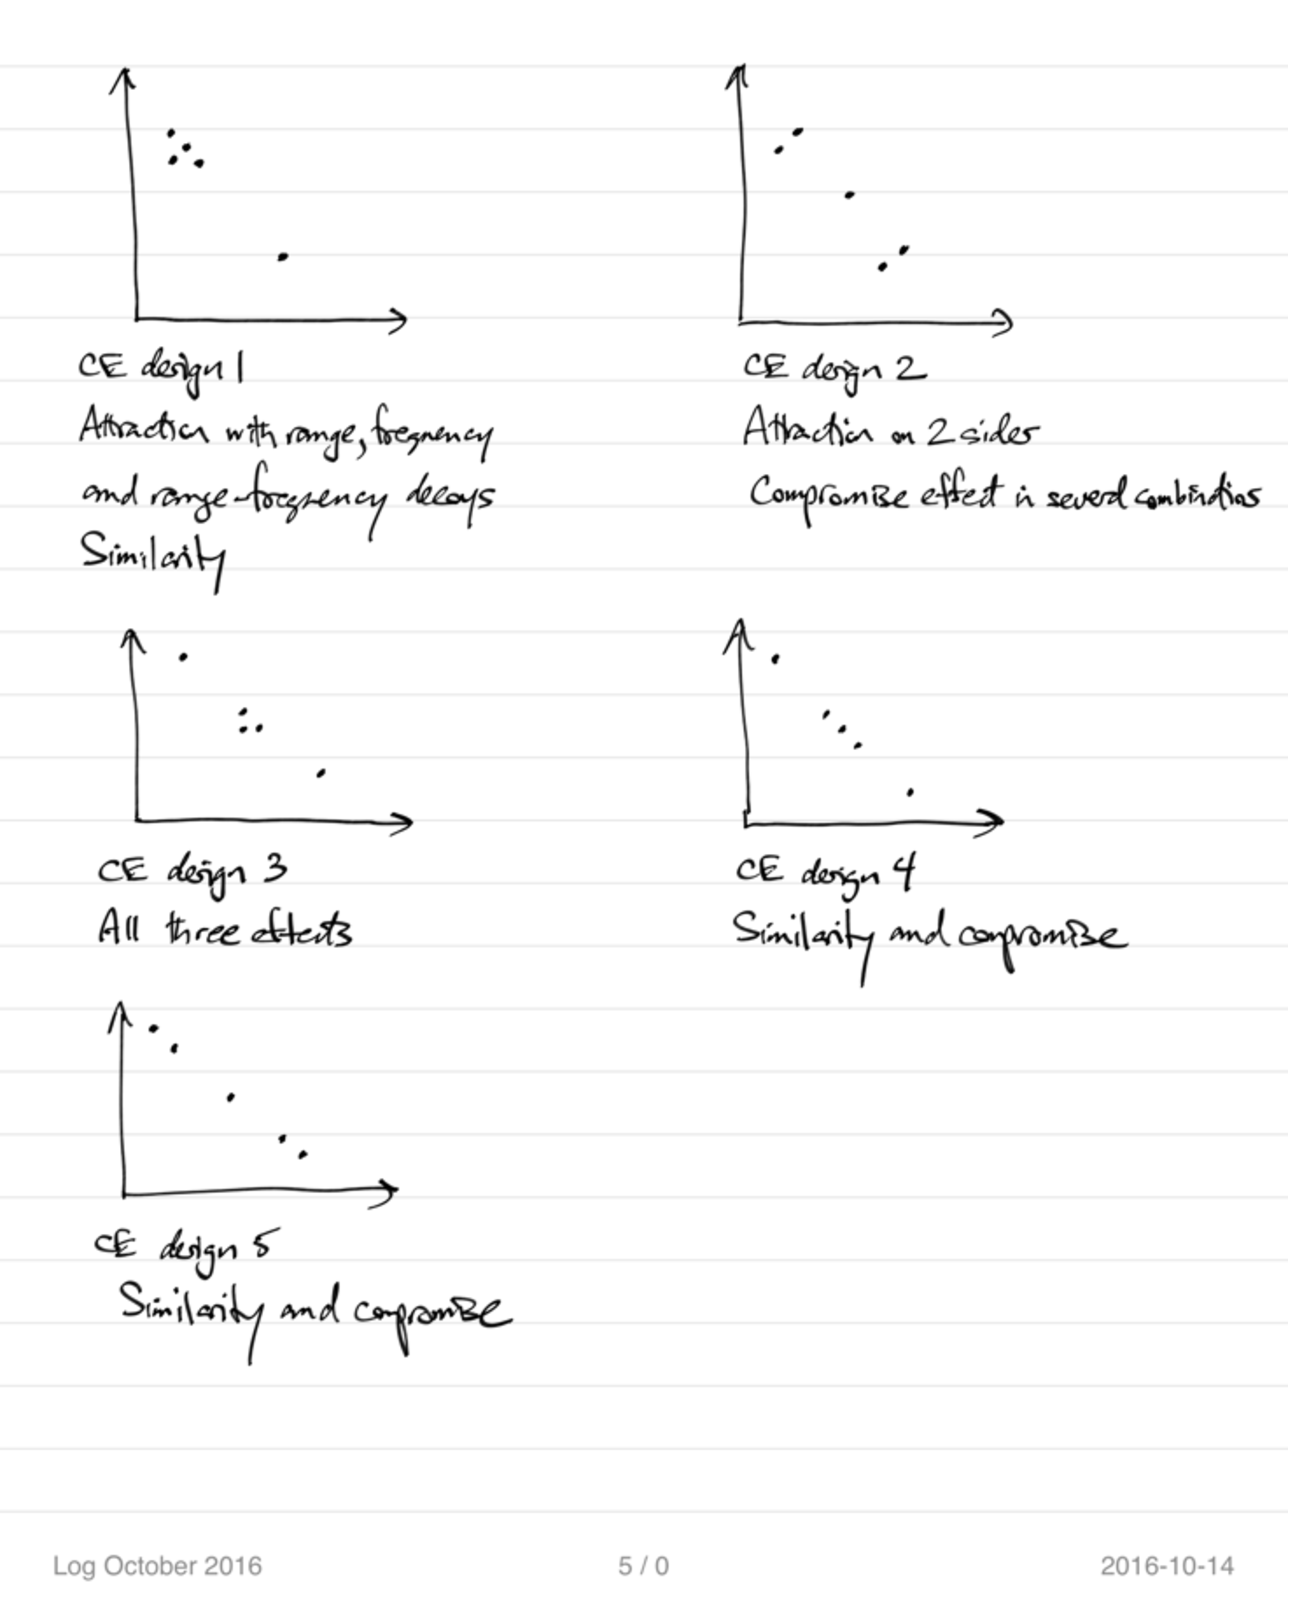
\includegraphics[height=10cm]{CEdesigns.pdf}
\end{figure}

% Ideas
% - perception of risk
% - rectangles
% - flights
% - moral judgments
% - political issues
% - job candidates
% - economic (or other) literacy
% - trivia

\end{document}
